\documentclass{article}

\usepackage{amsmath}
\usepackage{graphicx}
\usepackage{hyperref}

\begin{document}

\title{Putting Problem}
\author{Geoffrey Ulman\\
        Homework 5\\
        CSI747}
\date{October 2012}
\maketitle

\section{Physics Equations}\label{Physics Equations}

Let \(u(t)\) describe the position of a golf ball at time \(t\). Let \(v(t)\) describe the velocity of the golf ball, \(a(t)\) describe the acceleration, \(N(t)\) describe the normal vector force, and \(F(t)\) describe the rolling resistance force acting on the golf ball at time \(t\).

\begin{equation}\label{eq_normal}
n = \left( -\frac{df}{dx},-\frac{df}{dy}, 1 \right)
\end{equation}

If the surface is continuously differentiable, then the direction of the normal vector to the surface is given by equation \ref{eq_normal}.

\begin{equation}\label{eq_normal_norm}
\|n\|^2 = \left( \frac{df}{dx} \right)^2 + \left( \frac{df}{dy} \right)^2 + 1
\end{equation}

Thus, the squared norm of the normal vector is given by equation \ref{eq_normal_norm}.

\begin{eqnarray}\label{normalforce}
N_x = &- \frac{df}{dx} N_z \nonumber \\
N_y = &- \frac{df}{dy} N_z \nonumber \\
N_z = &m \frac{  \|g\| - a_x \frac{df}{dx} - a_y \frac{df}{dy}  +a_z  }{\|n\|^2}
\end{eqnarray}

Using the normal vector definitions above, and applying Newton's second law (force equals mass times acceleration) in the \(x\), \(y\), and \(z\) directions, we can describe the normal force acting on the ball via equation \ref{normalforce}.

\begin{eqnarray}\label{eq1}
N_x + F_x = ma_x \nonumber \\
N_y + F_y = ma_y
\end{eqnarray}

We can then use Newton's second law again to describe the interaction of the gravitational force, the normal force, and the resistance (or friction) forces acting on the ball.

\section{Discretization}\label{Discretization}

To model the above equations in AMPL, the problem was divided into \(n\) time steps with variable \(tf\) representing the unknown final time. Velocity was modeled as the difference in the ball's position at adjacent steps divided by the time difference between steps. Acceleration was similarly modeled and indexed such that indices for position and acceleration corresponded to values for the same time step. Velocity values were averaged to arrive at velocity values corresponding to the same time steps as the position and acceleration values.

\section{AMPL Model}\label{AMPL Model}

\begin{verbatim}

reset;

model;

# gravitational force in ft/s^2 
param g  := 32.174;

# mass of golf ball
param m := 0.01;

# surface normal coefficient
param mu := 0.25;

# initial position of ball
param x0 := 1;
param y0 := 2;

# position of cup
param xf := 1;
param yf := -2;

# discretization factor
param n := 50;

# final moment of time
var tf >= 0, <=30, := 3;

# position of ball
# set the initial values to form an evenly spaced line between
# the start and end positions (arbitrary, but reasonable initial values)
var x {j in 0..n} := j * ( xf - x0 ) / n;
var y {j in 0..n} := j * ( yf - y0 ) / n;
var z {j in 0..n} = 0.1 * ( x[j]^2 + y[j]^2 );

# derivative with respect to time of ball position
var dx {j in 0..n} = 0.2 * x[j];
var dy {j in 0..n} = 0.2 * y[j];

# squared normal vector norm
var norm_n_sq {j in 0..n} = dx[j]^2 + dy[j]^2 + 1;

# velocity of ball
var vx {j in 1..n} = ( x[j] - x[j-1] ) / ( tf / n );
var vy {j in 1..n} = ( y[j] - y[j-1] ) / ( tf / n );
var vz {j in 1..n} = ( z[j] - z[j-1] ) / ( tf / n );

var v_avg_x {j in 1..n-1} = ( vx[j] + vx[j+1] ) / 2;
var v_avg_y {j in 1..n-1} = ( vy[j] + vy[j+1] ) / 2;
var v_avg_z {j in 1..n-1} = ( vz[j] + vz[j+1] ) / 2;

# norm of velocity vector
var v_norm {j in 1..n} = sqrt( vx[j]^2 +
                               vy[j]^2 +
                               vz[j]^2 );


var v_avg_norm {j in 1..n-1} = sqrt( v_avg_x[j]^2 +
                                     v_avg_y[j]^2 +
                                     v_avg_z[j]^2 );

# acceleration of ball
# (see velocity_x and velocity_y constraints)
var ax {j in 1..n-1} = ( vx[j+1] - vx[j] ) / ( tf / n );
var ay {j in 1..n-1} = ( vy[j+1] - vy[j] ) / ( tf / n );
var az {j in 1..n-1} = ( vz[j+1] - vz[j] ) / ( tf / n );

# normal force
var Nz {j in 1..n-1} = m * ( ( g - ax[j] * dx[j] -
                               ay[j] * dy[j] + az[j] ) /
                               norm_n_sq[j] );

var Nx {j in 1..n-1} = -dx[j] * Nz[j];
var Ny {j in 1..n-1} = -dy[j] * Nz[j];

# norm of normal force
var N_norm {j in 1..n-1} = sqrt( Nx[j]^2 + Ny[j]^2 + Nz[j]^2 );

# resistance force
var Fx {j in 1..n-1} = -mu * N_norm[j] * ( v_avg_x[j] / v_avg_norm[j] );
var Fy {j in 1..n-1} = -mu * N_norm[j] * ( v_avg_y[j] / v_avg_norm[j] );

minimize final_velocity: vx[n]^2 + vy[n]^2 + vz[n]^2;

s.t. initial_position_x: x[0] = x0;
s.t. initial_position_y: y[0] = y0;

s.t. final_position_x: x[n] = xf;
s.t. final_position_y: y[n] = yf;

s.t. bounding_box {j in 0..n}: 4 * x[j] + y[j] <= 16;

# Newton's laws F = ma
s.t. newton_x {j in 1..n-1}: Nx[j] + Fx[j] = m * ax[j];
s.t. newton_y {j in 1..n-1}: Ny[j] + Fy[j] = m * ay[j];

option solver loqo;

option loqo_options "iterlim=8000";

solve;

display x;
display y;
display z;

display vx[1];
display vy[1];
display vz[1];

display v_norm[1];
display v_norm[n];

\end{verbatim}

\section{AMPL Results}\label{AMPL Results}

\begin{figure}
\centering
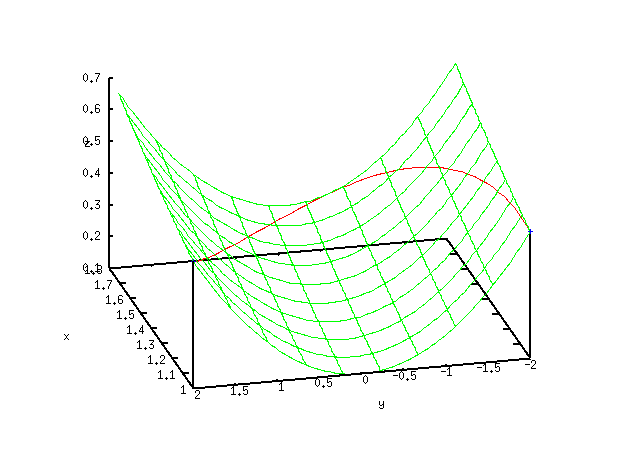
\includegraphics[width=0.9\textwidth]{ball_path.png}
\caption{Ball Path and 3D Putting Green Surface}
\vspace{2 cm}
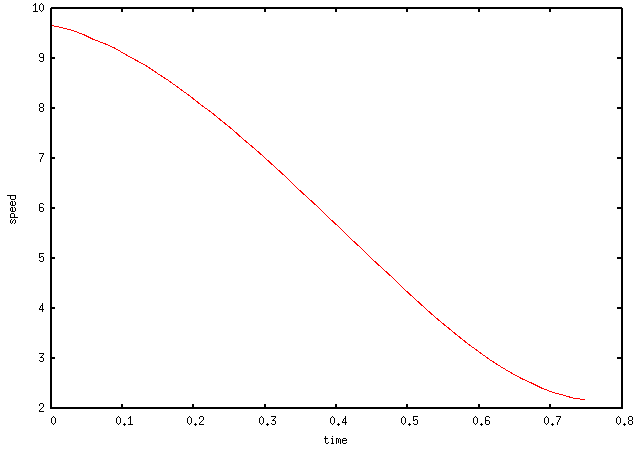
\includegraphics[width=0.9\textwidth]{ball_speed.png}
\caption{Ball Speed Over Time}
\end{figure}

\begin{verbatim}

LOQO 6.07: iterlim=8000
LOQO 6.07: optimal solution (26 iterations, 26 evaluations)
primal objective 4.785488588
  dual objective 4.785488675
x [*] :=
 0 1          9 1.49349   18 1.70248   27 1.66294   36 1.45356   45 1.16397
 1 1.06833   10 1.53069   19 1.70913   28 1.64645   37 1.42369   46 1.13068
 2 1.13346   11 1.56431   20 1.71276   29 1.62799   38 1.39295   47 1.09757
 3 1.1953    12 1.59436   21 1.71349   30 1.60766   39 1.36148   48 1.0647
 4 1.25376   13 1.62088   22 1.71141   31 1.58559   40 1.32939   49 1.03216
 5 1.30879   14 1.64391   23 1.70664   32 1.56192   41 1.29681   50 1
 6 1.36031   15 1.66352   24 1.69929   33 1.53675   42 1.26386
 7 1.40829   16 1.67976   25 1.68948   34 1.51022   43 1.23066
 8 1.45268   17 1.69272   26 1.67732   35 1.48245   44 1.19733
;

y [*] :=
 0  2           11  0.617563    22 -0.625028    33 -1.50053     44 -1.935
 1  1.87712     12  0.494249    23 -0.72189     34 -1.55835     45 -1.95345
 2  1.7529      13  0.372409    24 -0.815505    35 -1.61245     46 -1.9687
 3  1.6276      14  0.252267    25 -0.905786    36 -1.66283     47 -1.98086
 4  1.50148     15  0.134033    26 -0.992654    37 -1.7095      48 -1.99005
 5  1.37479     16  0.0179076   27 -1.07604     38 -1.75247     49 -1.99638
 6  1.2478      17 -0.0959234   28 -1.15589     39 -1.79178     50 -2
 7  1.12077     18 -0.207286    29 -1.23214     40 -1.82747
 8  0.993978    19 -0.316019    30 -1.30476     41 -1.85957
 9  0.867674    20 -0.421976    31 -1.37371     42 -1.88815
10  0.742119    21 -0.525019    32 -1.43898     43 -1.91327
;

z [*] :=
 0 0.5        11 0.282845   22 0.331958   33 0.461318   44 0.517783
 1 0.466489   12 0.278627   23 0.343374   34 0.470923   45 0.517078
 2 0.435739   13 0.276594   24 0.355263   35 0.479766   46 0.515421
 3 0.407783   14 0.276609   25 0.367478   36 0.487786   47 0.512845
 4 0.382636   15 0.278525   26 0.379877   37 0.494928   48 0.509387
 5 0.360297   16 0.282192   27 0.392323   38 0.501148   49 0.505091
 6 0.340744   17 0.28745    28 0.404688   39 0.506411   50 0.5
 7 0.32394    18 0.29414    29 0.416851   40 0.510691
 8 0.309828   19 0.302098   30 0.428697   41 0.513971
 9 0.298337   20 0.311161   31 0.44012    42 0.516244
10 0.289377   21 0.321168   32 0.451024   43 0.517511
;

vx[1] = 4.56243

vy[1] = -8.20536

vz[1] = -2.23766

v_norm[1] = 9.65147

v_norm[n] = 2.18758

\end{verbatim}

\section{Discussion}\label{Discussion}

As indicated by the AMPL results above, the ball arives at the hole with a minimum possible speed of \(2.19\) when hit with an initial velocity vector of approximately \(\left( 4.56, -8.21, -2.24 \right)\).

The direction of the ball is somewhat counterintuitive. Because of the putting green is an inverted bowl shape, the ball must be hit in order to curve around the outside of the bowl instead of more directly toward the hole in order to arrive with minimum speed.

\end{document}
